\section*{Einleitung}
Die Erfindung des \glqq scanning tunneling microscope\grqq (STM) machte erstmals die atomare Auflösung von Oberflächen möglich.
Das grundlegende Konzept beruht dabei auf der Nutzung des stark abstandsabhängigen Tunnelstroms zwischen der Probe und einer scharfen Spitze.
Eben dieses Funktionsprinzip stellt eine intrinsische Begrenzung des STM dar.
Nur metallische Oberflächen können mit dieser Methode betrachtet werden.
Das \glqq atomic force microscope\grqq (AFM) macht es möglich auch nicht-leitende Materialien aufzulösen, da hierbei die Kraft zwischen Spitze und Probe bei Distanzen von ca. $\SI{1}{nm}$ ausgenutzt wird.
Es bildet die Weiterentwicklung des STM und des stylus profilometers, dessen Auflösung durch die Größe seiner Spitze ($\sim 1\mu m$) begrenzt ist.
Ein weiterer gravierender Vorteil gegenüber dem STM besteht beim AFM darin, dass es auch an der Luft und bei Raumtemperatur bedient werden kann.
Vor diesem Hintergrund wurden in diesem Experiment mehrere Proben unter diesen Normalbedingungen vermessen, um die Leistungskraft dieses Verfahrens bei der Untersuchung ihrer Topographien aufzuzeigen.

\section{Theorie}
\subsection{Kraft zwischen Spitze und Probe}
    Bei einem Spitzen-Proben Abstand von $> \SI{1}{nm}$ stellen die attraktiven langreichweitigen Kräfte, die unter der Van-der-Waals-Wechselwirkung zusammengefasst werden können, die größte Kraft dar. Diese beruhen jeweils auf der Coulomb-Wechselwirkung.
    \hspace{3cm}
    \begin{description}
        \item[Dipol-Dipol-WW:]  Diese Kraft bildet sich zwischen zwei permanent polaren Molekülen aus, die einander anziehen.
        \item[Induktions-WW:]  Kraft zwischen polarem und neutralem Molekül, wobei das Polare dem Neutralen ein magnetisches Dipolmoment induziert.
        \item[London-Dispersions-WW:]  Diese Kraft wirkt zwischen zwei neutralen Molekülen. Durch Fluktuationen entstehen spontane elektrische Dipole, die sich gegenseitig anziehen.
    \end{description}
    Die letzte überwiegt meist gegenüber den anderen beiden Kräften. \\
    Unter der Annahme zweier Edelgsatome lässt sich ihr Wechselwirkungspotential mit der Abstandsabhängigkeit
    \begin{equation*}
        V_{\mathrm{VdW}(r)} \propto -\frac{1}{r^6}
    \end{equation*}
    ausdrücken.

    Bei einem Spitzen-Proben Abstand von $< \SI{1}{nm}$ entstehen kurzreichweitige WW aufgrund des Überlapps zwischen den elektronischen Zustandsdichten.
    Wird der Abstand in fallender Ordnung durchlaufen, so ist die Wechselwirkung erst attraktiv, da durch den Überlapp der äußeren offenen Schalen chemische Bindungen entstehen, die die Gesamtenergie minimieren. \\
    \setlength{\columnsep}{10pt}
    \begin{wrapfigure}{r}{0.4\textwidth}
        \centering\captionsetup{margin={0.5cm,-1cm}, format=plain}
        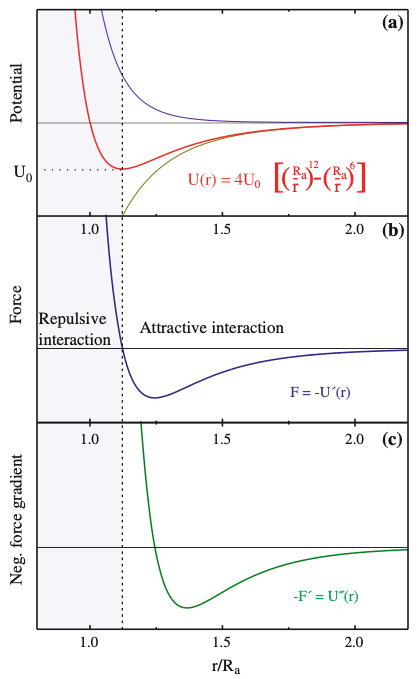
\includegraphics[width=0.48\textwidth]{bilder/Lennard_Jones_Potential.png}
        \caption{Hier ist das Lennard-Jones-Potential, seine zugehörige Kraft und dessen negierte Ableitung dargestellt. \cite{voigtlaender}} \vspace*{-0.5cm}
        \label{fig:Lennard_Jones_Potential}
    \end{wrapfigure}
    Dann kommen sich die Spitze und Probe so nah, dass die geschlossenen Orbitale überlappen.
    Die kernnahen Elektronen müssen aufgrund des Pauli-Verbotes in höhere Zustände ausweichen.
    D.h. sie müssen effektiv weiter vom Kern des anderen, an der Wechselwirkung beteiligten, Atoms entfernt sein.
    Diese Wechselwirkung wird durch
    \begin{equation}
        V_{\mathrm{Pauli}(r)} \propto \frac{1}{r^{12}}
    \end{equation}
    beschrieben.
    Die gesamte Wechselwirkung zwischen Sptize und Probe lässt sich also in erster Näherung durch das Lennard-Jones-Potential
    \begin{equation}
        U_{\mathrm{LJ}}(r) = 4 U_0 \left[\left(\frac{R_a}{r}\right)^{12} - \left(\frac{R_a}{r}\right)^6\right]
        \label{eqn:Lennard_Jones_Potential}
    \end{equation}
    schreiben, wobei $U_0$ die Tiefe des Potentialminimums ist und $R_a$ der Abstand ist, bei dem $V(r) = 0$ gilt.
    Im obersten Graphen in \autoref{fig:Lennard_Jones_Potential} ist das Potential mit den soeben beschriebenen Parametern zu erkennen.
    Die gestrichelte Linie grenzt den repulsiven von dem attraktiven Effekt der Wechselwirkung ab.

    Eine weitere Kraft, die bei der Wechselwirkung zwischen Spitze und Probe eine große Rolle spielt, ist die elektrostatische Wechselwirkung.
    Sie entsteht durch unterschiedliche Austrittsarbeiten bzw. durch eine Ladung auf der Spitze und Probe, sodass eine weitere Kraft auf die Spitze wirkt und auf die Kraft-Abstandskurve Einfluss nimmt.
    Da dies beim AFM nicht erwünscht ist wird eine Bias-Spannung angelegt, die die Potentialdifferenz ausgleichen soll nach 
    \begin{equation}
        \Delta V = V_{\mathrm{bias}} - \Delta \Phi \cdot e = 0 \quad \Leftrightarrow \quad V_{\mathrm{bias}} = \Delta \Phi \cdot e \;.
    \end{equation}
    Die Kraft zwischen Spitze und Probe ist näherungsweise gegeben als
    \begin{equation}
        F_{el}(z) \approx -\pi \epsilon_0 \frac{R}{z} \cdot \Delta V^2 \;,
    \end{equation}
    wenn die Spitze als Kugel auf einem Kegel und die Probe als unendliche Ebene betrachtet wird, wobei $R$ der Radius der Kugel ist.
    Es ist zu erkennen, dass die Kraft als Funktion der Bias-Spannung $F_{el}(V_{\mathrm{bias}})$ eine umgedrehte Parabel mit einem Maximum an der Stelle $\Delta \Phi \cdot e$ darstellt.
    Die Differenz Austrittsarbeit zwischen Spitze und Probe kann also durch Auftragen der Kraft gegen die Bias-Spannung bestimmt werden.

\subsection{Snap-to-Contact}
    Ein wichtiges Konzept um die Funktionsweise von AFM-Messungen im Contact-Mode zu verstehen ist der Snap-to-Contact bzw. Snap-out-of-Contact der Spitze zur Probenoberfläche.
    Im dynamischen Modus wird dieser Snap-to-Contact gemieden, da die Oszillation des Cantilevers sonst wegen des schmalen Potentialminimums gestoppt werden würde, mehr dazu in \autoref{sec:messmodi}.
    Aus diesem Grund werden die Bedingungen für den Snap-to-Contact hier betrachtet.

    Der Cantilever an dem die Spitze befestigt ist kann als Feder mit dem Potential
    \begin{equation}
        U_{\mathrm{cant}}(z) = \frac{1}{2}k(z - z_0)^2
        \label{eqn:harm_Potential}
    \end{equation}
    aproximiert werden.
    Um den Snap-to-Contact zu erklären werden nun aus den beiden in \autoref{fig:Lennard_Jones_Potential} dargestellten Potentialen \eqref{eqn:Lennard_Jones_Potential} und \eqref{eqn:harm_Potential} die zugehörigen Kräfte abgeleitet und in die Betrachtung einbezogen.
    Dies ergibt die Kraft-Abstands-Kurven, wie in \autoref{fig:Snap_to_Contact_Kraft} zu erkennen.
    \begin{figure}
        \centering
        \begin{subfigure}{0.49\textwidth}
            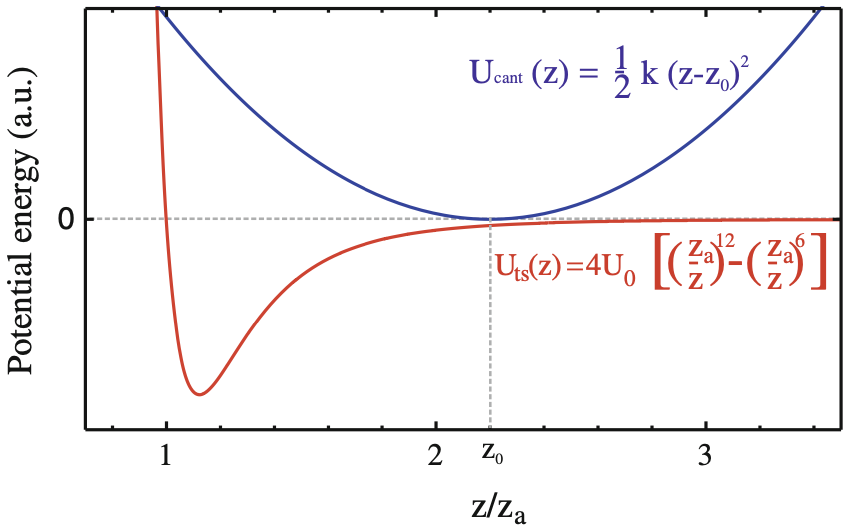
\includegraphics[width = \textwidth]{bilder/Snap_to_Contact_Potential.png}
            \caption{}
            \label{fig:Snap_to_Contact_Potential}
        \end{subfigure}
        \hfill
        \begin{subfigure}{0.49\textwidth}
            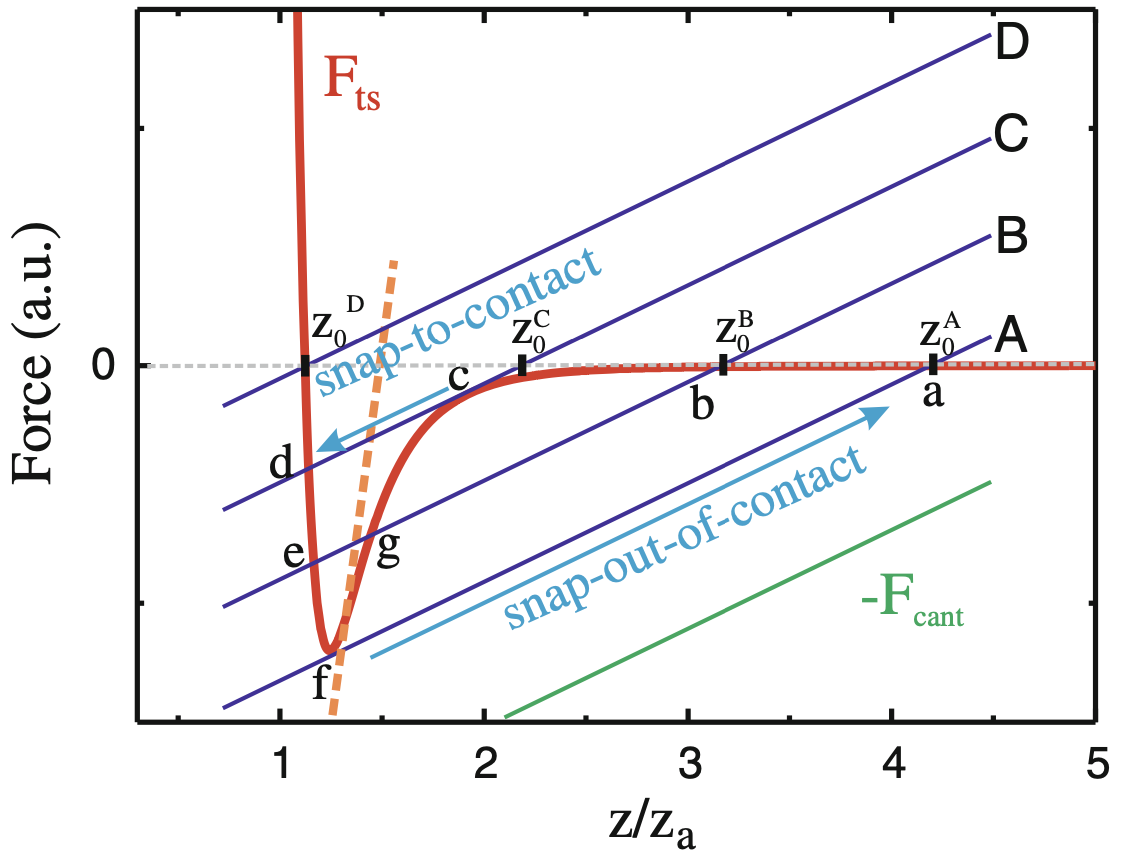
\includegraphics[width = \textwidth]{bilder/Snap_to_Contact_Kraft.png}
            \caption{}
            \label{fig:Snap_to_Contact_Kraft}
        \end{subfigure}
        \caption{\textbf{(a)} Das Lennnard-Jones-Potential für die Spitzen-Proben-WW und ein harmonisches Potential für den Cantilever bei seiner Gleichgewichtsposition $z_0$ bei ausgeschalteter Spitzen-Proben-WW ist dargestellt. \textbf{(b)} Kraft-Abstands-Kurven für verschiedene $z_0$ anhand derer der Snap-to-Contact erklärt wird. \cite{voigtlaender}}
        \label{fig:Snap_to_Contact}
    \end{figure}
    \FloatBarrier
    Der Snap-to-Contact kommt dadurch Zustande, dass der Cantilever bei der Annäherung zur Probe aus einem Potentialminimum ins Nächste springt.
    Um also die Bedingung für diesen Sprung zu bestimmen, wird ein Extremwertproblem der Potentialfunktion
    \begin{equation}
        U(z) = U_{\mathrm{LJ}}(z) + U_{\mathrm{cant}}(z)
    \end{equation}
    gelöst. Die notwendige Bedingung lautet
    \begin{alignat}{2}
        && \frac{\partial U_{\mathrm{LJ}}}{\partial z} + k(z - z_0) &= 0 \nonumber\\
        \Leftrightarrow && F_{\mathrm{LJ}} &= -F_{\mathrm{cant}} \;.
    \end{alignat}
    Dieses Kräfte werden in \autoref{fig:Snap_to_Contact_Kraft} graphisch dargestellt.
    Dabei sind die blauen Geraden die negative Federkraft bei verschiedenen $z_0$. \\
    Die hinreichende Bedingung
    \begin{alignat}{2}
        && \frac{\partial U_{\mathrm{LJ}}^2}{\partial^2 z} + k &> 0 \nonumber\\[3pt]
        \Leftrightarrow && \frac{\partial F_{\mathrm{LJ}}}{\partial z} &< k
    \end{alignat}
    bestimmt, ob es sich bei einem Schnittpunkt des roten und blauen Graphen um ein Minimum handelt.
    In \autoref{fig:Snap_to_Contact_Kraft} ist zu erkennen, dass sich der Cantilever bei kleinen Auslenkungen vor dem Punkt c immer im Potentialminimum an der Gleichgewichtsposition $z_0$ befindet.
    Doch wird der Cantilever noch näher an die Probe rangebracht, gibt es plötzlich nur noch ein Minimum an der fallenden Flanke des roten Graphen, in das der Cantilever nun springt.

    Der Snap-out-of-Contact passiert bei größeren Spitzen-Proben-Abständen als $z_0^{\mathrm{A}}$ gibt es auch plötzlich nur noch ein Minimum und es geschieht ein Sprung aus Punkt f nach Punkt a.

    Zum Einen kann ein größerer Gleichgewichtsabstand des Cantilevers gewählt werden (grüne Gerade), um den Snap-to-Contact im dynamischen Modus zu verhindern.
    Zum Anderen ist es möglich die Federkonstante $k$ so groß zu wählen, dass die Steigung der roten Kurve bei jedem $z_0$ kleiner ist als die der blauen Geraden ist (orange gestrichelte Gerade).
    Das führt dazu, dass es nur einen Schnittpunkt im Graphen bzw. nur ein Potentialminimum gibt und so auch kein Sprung zwischen zwei Minimas passiert.

\subsection{Kraft-Abstands-Kurven}
    \begin{figure}[ht]
        \centering\captionsetup{format=plain}
        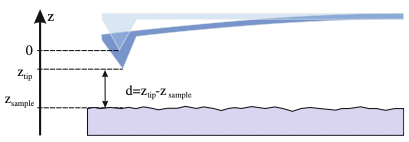
\includegraphics[width=0.55\textwidth]{bilder/Cantilever_Auslenkung.png}
        \caption{Das ist die Visualisierung der in der Kraft-Abstands-Kurve geplotteten Koordinaten. \cite{voigtlaender}}
        \label{fig:Cantilever_Auslenkung}
    \end{figure}
    \FloatBarrier
    Kraft-Abstands-Kurven werden gemessen, indem die Probe an den Cantilever angenähert wird und seine Auslenkung aufgenommen wird, die über das Hook'sche Gesetz proportional zur Kraft zwischen Probe und Spitze ist.
    Daraus lassen sich Größen wie die maximale Adhäsionskraft und die Elastizität der Probe bestimmen.
    Es wird also die Position der Probe $z_{\mathrm{sample}}$ und die Position der Spitze $z_{\mathrm{tip}}$ gegeneinander aufgetragen.
    Beide Koordinaten sind zum besseren Verständnis in \autoref{fig:Cantilever_Auslenkung} graphisch dargestellt.
    Eine ideale Kraft-Abstands-Kurve ist in \autoref{fig:Kraft_Abstands_Kurve} zu sehen.
    Nach dem Snap-to-Contact von Punkt c zu Punkt d, bewegen sich Spitze und Probe gemeinsam weiter, weil die Probe die Spitze nach oben auslenkt.
    Eine weiche Probe würde eindellen und die Kurve würde zumindest in der Nähe von Punkt d eine Steigung kleiner eins besitzen, woraus auf die elastischen Eigenschaften der Probe geschlossen werden kann.
    \begin{figure}[ht]
        \centering\captionsetup{format=plain}
        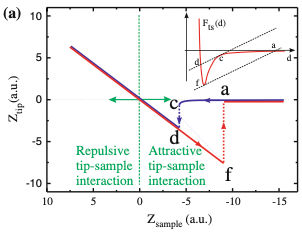
\includegraphics[width=0.5\textwidth]{bilder/Kraft_Abstands_Kurve.png}
        \caption{Eine schematische Kraft-Abstands-Kurve, wobei blau die Annäherung von Spitze und Probe und rot ihre Entfernung bedeutet. \cite{voigtlaender}}
        \label{fig:Kraft_Abstands_Kurve}
    \end{figure}
    \FloatBarrier

\subsection{Cantilever und Spitze}
\label{sec:cantilever}
    \setlength{\columnsep}{25pt}
    \begin{wrapfigure}{r}{0.4\textwidth} \vspace*{-0.5cm}
        \centering\captionsetup{margin={0.5cm,-1cm}, format=plain}
        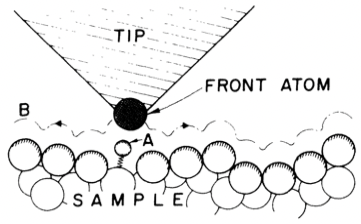
\includegraphics[width=0.4\textwidth]{bilder/Federkraftkonstante.png}
        \caption{Das ist die schematische Darstellung einer Spitzen-Proben-WW, als WW des Atoms A und der Spitze. \cite{atomic_force_microscope}} \vspace*{-0.3cm}
        \label{fig:Federkraftkonstante}
    \end{wrapfigure} 
    \FloatBarrier
    Die Maße und Federkonstante des Cantilevers hängen von den Kräften zwischen Spitze und Probe ab, die bei der AFM-Messung ausgenutzt werden.
    
    Da eine atomare Auflösung erreicht werden soll, muss der Cantilever sensitiv genug sein, um durch die Wechselwirkung zwischen zwei einzelnen Atomen ausgelenkt zu werden.
    Als Aproximation wird das Atom A in \autoref{fig:Federkraftkonstante} als ein harmonischer Oszillator mit einer Vibrationsfrequenz von $\omega_{\mathrm{vib}} = 10^{13}\,$Hz und einer Atommasse von $m = 10^{-25}\,$kg angenommen.
    Beides sind typische Werte für Festkörper.
    Damit ergibt sich eine kleine Federkonstante von
    \begin{equation}
        \omega_{\mathrm{vib}} = \sqrt{\frac{k}{m}} \qquad \Leftrightarrow \qquad k = \omega_{\mathrm{vib}}^2 m \approx 10\,\si{Nm^{-1}}
    \end{equation}
    für die Atombindung zwischen Atom A und seinen Nachbarsatomen.
    Mit typischen Atomabständen von ca. $10^{-10}\,$m, erhält man in erster Näherung mit dem Hookschen Gesetz Atomkräfte im Bereich von Nanonewton.
    Um sensitiv gegenüber diesen Kräften zu sein, sollte der Cantilever eine Federkonstante in der gleichen Größenordnung wie die Atombindungen besitzen.
    Im Umkehrschluss heißt das, dass dieser auch im Angströmbereich ausgelenkt wird.
    Die erste Bedingung an den Cantilever ist also, dass er eine kleine Federkraftkonstante haben bzw. weich sein soll.

    Außerdem sollte das AFM vor externen Vibrationen, wie z.B. Gebäudeschwingungen von ca. \SI{100}{Hz}, geschützt sein.
    Dies wird durch eine sehr hohe Resonanzfrequenz des Cantilevers $\gg \SI{10}{kHz}$ erreicht, was die zweite Bedingung an den Cantilever darstellt.
    Zusätzlich sind dadurch hohe Scangeschwindigkeiten möglich.
    
    Beide Bedingungen können nach $\omega_{\mathrm{cant}} = \sqrt{\frac{k}{m}}$ nur gleichzeitig erfüllt sein, wenn die Masse des Cantilevers sehr klein ist.
    Für eine Frequenz von $\omega_{\mathrm{cant}} = \SI{100}{kHz}$ und eine von Federkonstante $k = \SI{10}{Nm^{-1}}$ muss der Cantilever ca. $\SI{1}{\mu m}$ wiegen, um beide Bedingungen zu erfüllen.

    Die Spitze sollte einen möglichst kleinen Spitzenradius und einen schmalen Abschluss besitzen, da die Strukturen in den AFM-Bilder immer um die Spitzenbreite verbreitert werden.
    Das gemessene Bild ist also eine Faltung zwischen Spitze und Probentopographie, wie in \autoref{fig:Spitze_Probe_Faltung} zu sehen ist.
    \begin{figure}[ht]
        \centering\captionsetup{format=plain}
        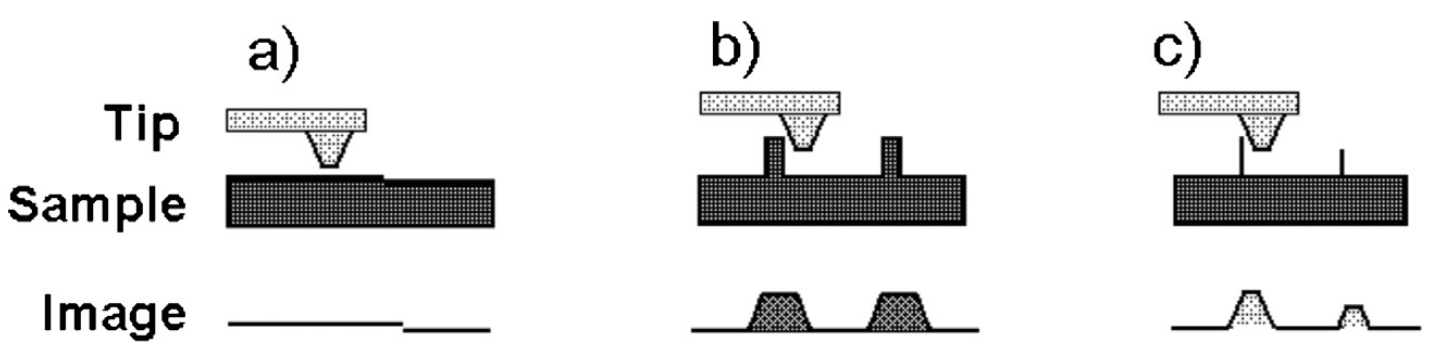
\includegraphics[width=0.8\textwidth]{bilder/Spitze_Probe_Faltung.png}
        \caption{Es sind drei Fälle aufgezeigt: \textbf{(a)} eine scharfe Spitze ist nicht notwendig, \textbf{(b)} eine scharfe Spitze und die Spitzenform zur topographischen Interpretation ist notwendig, \textbf{(c)} Selbstabbild der Spitze durch schärfere Strukturen. \cite{AFM_image_artifacts}}
        \label{fig:Spitze_Probe_Faltung}
    \end{figure}

\subsection{Detektion}
\label{sec:detektion}
    Wie in \autoref{sec:cantilever} bereits erklärt, wird der Cantilever bei der Messung im Angströmbereich ausgelenkt.
    Die Detektionsmethode sollte das System möglichst nicht stören z.B. durch Kraftauswirkung auf den Cantilever oder Erwärmung.
    Im folgenden werden ein paar verschiedene Methoden angesprochen.

    \newpage
    \subsubsection*{Laserreflektion}
        % \setlength{\columnsep}{50pt}
        \begin{wrapfigure}{r}{0.4\textwidth}
            \centering\captionsetup{margin={0.5cm,-1cm}, format=plain}
            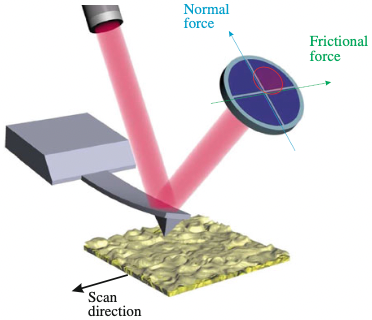
\includegraphics[width=0.4\textwidth]{bilder/Viersegmentphotodiode.png}
            \caption{Schematische Darstellung der Laserreflektionsmethode. \cite{voigtlaender}} \vspace*{-0.3cm}
            \label{fig:Viersegmentphotodiode}
        \end{wrapfigure}
        \FloatBarrier
        Diese Methode wird aufgrund ihres einfachen Aufbaus und ihrer Entkopplung vom System am häufigsten benutzt.
        Die einzige Voraussetzung ist dabei eine spiegelnde Rückseite des Cantilevers.
        Ein Laserstrahl wird auf diese Rückseite fokussiert, wird dort reflektiert und trifft auf eine Vier-Segment-Photodiode.
        Die Differenz zwischen den, durch das reflektierte Laserlicht zustandekommenden, Signalen auf den unteren und oberen beiden Photodioden ist proportional zur Auslenkung des Cantilevers.
        Durch die zusätzliche Aufteilung der Dioden in Links und Rechts ist es außerdem möglich die Torsion des Cantilevers zu messen.
        Die Torsion ist proportional zu den Reibungskräften, die beim Bewegen der Spitze aufkommen.
        Dies ist nützlich um die Degradation der Probe nach mehrmaligem Abrastern untersuchen zu können.
        Es wird die Probe und nicht der Cantilever bewegt, um den Laser nicht nach jeder Bewegung neu fokussieren zu müssen.

    \subsubsection*{Interferometrie}
        Eine aufbautechnisch aufwändigere optische Methode ist die Interferometriemethode zur Messung der Auslenkung des Cantilevers.
        Wie auch bei der anderen optischen Methode der Laserreflektion geht die Interaktion mit dem Cantilever nur vom Strahlungsdruck im Bereich von $10^{-12}\,$N aus, was vernachlässigbar klein ist.
        Außerdem ist hier die Größe des Cantilevers durch die Wellenlänge nach unten beschränkt, denn das Beugungslimit besagt, dass Licht nicht mehr als auf ca. seine halbe Wellenlänge fokussiert werden kann.
        Dies begrenzt somit die Sensitivität bzw. die Entkopplung von mechanischen Störungen, wie in \autoref{sec:cantilever} besprochen und damit die mögliche Auflösung.
        Ein weiteres Limit der optischen Methoden bildet das Schrotrauschen der Detektoren bei hohen Scangeschwindigkeiten.
        Schrotrauschen entsteht dadurch, dass nur paar Photonen in der kurzen Zeit einer Messung auf die Detektoren treffen und die gemessene Intensität pro Messung stark fluktuiert, nach dem Gesetz der großen Zahlen.

        Es wird der Phasenabstand zwischen dem am ausgelenkten Cantilever reflektierten Strahl und einem Referenzstrahl durch Interferenz bestimmt.
        Daraus kann wiederum die Auslenkung des Cantilevers errechnet werden.

    \subsubsection*{STM}
        Eine weitere Möglichkeit bietet die Messung mithilfe eines STM.
        Durch die extreme räumliche Nähe und einer Potentialdifferenz der STM-Spitze zum Cantilever fließt ein extrem abstandsabhängiger Tunnelstrom, der es ermöglicht eine Sensitivität von $0,01\,\si{\angstrom}$ zu erreichen.
        Typische Tunnelströme sind jedoch sehr klein (nA) und bedürfen großer Verstärkung.
        Im dynamischen Messmodi, wo der Cantilever mit Resonanzfrequenzen von $30-100\,$kHz oszilliert würde also kein nennenswerter Tunnelstrom gemessen werden.
        Das Gleiche gilt für hohe Scangeschwindigkeiten.
        Aus diesem Grund diese Methode nur für statische Messungen verwendet.
        Zudem muss der Cantilever sauber sein, um zu verhindern, dass der Tunnelstrom durch Kontaminationen abgeschirmt wird und die STM-Spitze auf den Cantilever aufdrückt, um den Tunnelstrom aufrecht zu erhalten.
        Einen schwerwiegenden Nachteil bildet der komplizierte Aufbau, da das STM nur im UHV benutzt werden kann.
        Bei Messungen, die ohnehin im Vakuum und bei tiefen Temperaturen durchgeführt werden müssen, bietet sich diese Methode jedoch an, da optische Detektionsmethoden bei solch thermisch empfindlichen Systemen eine Erwärmung auslösen könnten.

\subsection{Messmodi}
\label{sec:messmodi}
    Insgesamt werden die verschiedenen Messmodi zur Aufnahme der AFM-Bilder in zwei Gruppen eingeteilt, die statischen und die dynamischen Modi.
    Bei den statischen Modi wird die Biegung des Cantilevers im Gleichgewichtszustand als Maß für die Stärke der Kraft zwischen Spitze und Probe genutzt.

    Der constant-force Modus ist die wahrscheinlich geläufigste statische Messmethode und wurde auch in dem vorliegenden Versuch verwendet.
    Während des Abrastern der Probe wird die Auslenkung des Cantilevers konstant gehalten, indem der Spitzen-Proben-Abstand über einen Feedbackloop kontinuirlich nachgeregelt wird.
    Zu Anfang der Messung muss deshalb zuerst ein Abstand gewählt werden, welcher eingehalten werden soll.
    Die Spitze kann entweder durch den Snap-to-Contact direkt auf der Probe abgesetzt werden und man arbeitet im repulsiven contact-Bereich, oder der Abstand wird so gewählt, dass man sich noch im attraktiven non-contact-Bereich befindet.
    Der contact-Modus verursacht größere Schäden an der Probe, was vor allem bei weicher biologischer Materie vermieden werden soll.
    Falls die Probe durch einen Flüssigkeitsfilm kontaminiert ist, nehmen Messungen im non-contact-Modus nicht die unterliegende Oberfläche, sondern die adsorbierte Kontamination auf.

    Im constant-height Modus wird die Spitze bei einer konstanten Höhe gehalten und die Auslenkung des Cantilevers wird aufgenommen.
    Da die Scanzeit hierbei nicht durch die elektronischen Bauteile begrenzt ist, können sehr hohe Scangeschwindigkeiten erreicht werden.
    Diese Methode kann, jedoch nur bei kleinen zuscannenden Bereichen angewendet werden, da die Wellung der Probe sonst zu groß sein könnte.

    Die dynamischen Modi funktionieren nach dem Prinzip, dass der Cantilever nahe seiner Resonanzfrequenz zu Schwingungen angeregt wird.
    Dies wird meist durch ein kleines Piezoelement am Halter des Cantilevers erreicht.
    Mit einer Feedbackschleife wird die Amplitude bzw. die Frequenz der Schwingung konstant gehalten, indem die Höhe des Cantilevers angepasst wird.
    Das Aufnehmen des Spitzen-Höhen-Abstandes an jedem Punkt der Probe erzeugt dann das AFM-Bild.

\subsection{Piezo}
\label{sec:piezo}
    Um die Probe in xy-Richtung abzurastern und die Spitze zur Probe in z-Richtung anzunähern werden Piezoelemente benutzt.
    Der inverse piezoelektrische Effekt in ferroelektrischen Nichtleitern führt zu einer Ausdehnung beim Anlegen einer elektrischen Spannung.
    Nur eine präzise Positionierung der Spitze relativ zur Probe macht die AFM-Messungen erst möglich.
    Dies wird jedoch durch nicht-lineares Verhalten des Piezos erschwert, wodurch Artefakte und Verzerrungen im aufgenommenen AFM-Bild enstehen und die Auswertung verkomplizieren.
    Somit ist es wichtig die Ursachen für solches Verhalten zu identifizieren, um die Bilder interpretieren zu können.
    
    \subsubsection*{Hysterese} \vspace*{-0.25cm}
        Die Hysteresekurve zwischen angelegter Spannung und der tatsächlichen Ausdehnung des Piezoelements wird durch ferroelektrische Domänen im Piezomaterial verursacht.
        Die Hysterese kommt genauer gesagt dadurch zustand, dass die Umgestaltung der Domänenstruktur energetische Barrieren darstellt und die Umorientierung der Domänen deshalb erst nach einem Aufstauen von elektrischer Energie passiert.
        Die Ausdehnung des Piezoelements ist damit ein Effekt, der auch von seinem Gedächtnis der Domänen abhängt.
        \begin{figure}[ht]
            \centering\captionsetup{format=plain}
            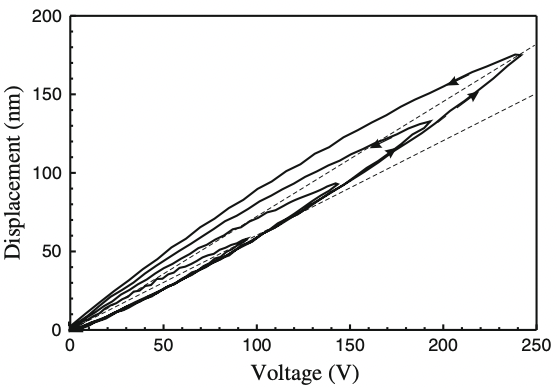
\includegraphics[width=0.5\textwidth]{bilder/Piezo_Hysterese.png}
            \caption{Es sind Hysteresen für verschiedene maximale Scanlängen bzw. angelegte Spannungen dargestellt. \cite{voigtlaender}}
            \label{fig:Piezo_Hysterese}
        \end{figure}
        Werden große Spannungsbereiche durchlaufen, um größere Proben abzurastern, erhöht sich die Hysterese wie in \autoref{fig:Piezo_Hysterese} gezeigt.
        Es wird eine Piezokonstante für jedes piezoelektrische Material, als durchschnittliches Verhältnis zwischen Ausdehnung und Spannung im Limit der kleinen Spannungsbereiche definiert.
        In \autoref{fig:Piezo_Hysterese} ist diese Piezokonstante die untere gestrichelte Gerade.
        Um größere Bereiche abzurastern und dabei die Hysterese zu minimieren werden also Materialien verwendet, die eine möglichst hohe Piezokonstante besitzen, sodass man nicht zu höheren Spannungsbereichen gehen muss.
        Das ist der Vorteil piezoelektrischer Keramiken gegenüber piezoelektrischen Kristallen.      

    \subsubsection*{Kriechen} \vspace*{-0.25cm}
        Da der inverse piezoelektrische Effekt auch von der Reorientierung von Domänen abhängt und dies eine gewisse Zeit in Anspruch nimmt, entsteht nach abrupten Änderungen in der angelegten Spannung ein Effekt genannt \glqq Creep\grqq.
        Die Dynamik des Piezos besteht aus dem ersten instantanen Teil und einem zweiten, sich über $\sim \SI{100}{s}$, hinziehenden Teil, wie in \autoref{fig:Piezo_Creep} zu sehen.
        \begin{figure}[ht]
            \centering\captionsetup{format=plain}
            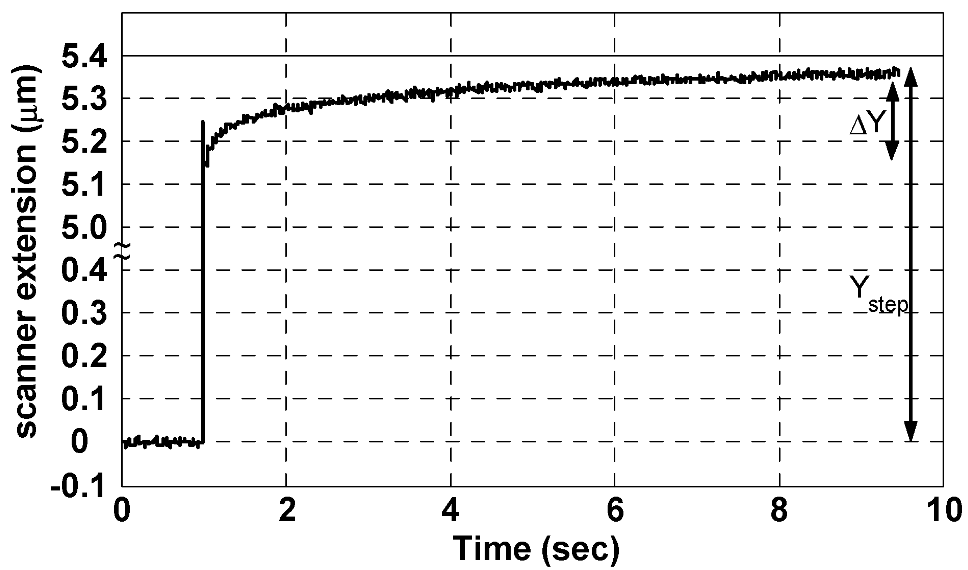
\includegraphics[width=0.5\textwidth]{bilder/Piezo_Creep.png}
            \caption{Es ist der Creep nach einem plötzlichen Spannungssprung dargestellt. $Y_{\mathrm{step}}$ ist dabei die gesamte und $\Delta Y$ die durch den Creep verursachte Verschiebung. \cite{Compensation_of_Scanner_Creep}}
            \label{fig:Piezo_Creep}
        \end{figure}
        Um Creep vorzubeugen werden Positionssensoren, siehe \autoref{sec:detektion}, in Verbindung mit einem Feedbackloop genutzt.
        

    \subsubsection*{Thermischer Drift} \vspace*{-0.25cm}
        Thermischer Drift ist nicht nur auf Piezoelemente beschränkt, sonder spielt bei allen mechanischen Komponenten des AFM ein Rolle, wie z.B. bei Cantilever, welcher durch seine extrem kleine Masse eine extrem kleine Wärmekapazität besitzt und sehr empfindlich gegenüber Erwärmung ist.
        Durch die Wahl von angrenzenden Materialien mit ähnlichen Wärmekapazitäten und einem symmetrischen Design des Piezoelementes kann der Einfluss des Drifts auf AFM-Bilder drastisch verringert werden.
        
    \vspace*{0.5cm}
    Aus diesen Gründen sollte vor jeder Anwendung des AFM an neuen Proben und in neuen Umgebungsbedingungen eine Kalibration anhand einer bereits bekannten Struktur durchgeführt werden.
    Wird z.B. ein Bild mit atomarer lateraler Auflösung aufgenommen, so sollte zur Kalibration eine bekannte atomar aufgelöste Struktur benutzt werden.
    Für die vertikale Kalibration werden normalerweise mono-atomige Stufen genutzt.
    Der Vorteil piezoelektrischer Kristalle wie z.B. Quarz ist, dass sie eine hohe Temperaturstabilität, schmale Hysterese und geringes Kriechen besitzen.